\documentclass[11pt, conference, letterpaper]{IEEEtran}

\usepackage{amsmath, amssymb, amsfonts}
\usepackage{graphicx}
\usepackage{algorithm}
\usepackage{algorithmic}
\usepackage{cite}
\usepackage{hyperref}

\begin{document}

\title{Kanade-Lucas-Tomasi (KLT) Feature Tracker: Theory, Implementations, and Performance Analysis}

\author{
\IEEEauthorblockN{Weston Scott}
\IEEEauthorblockA{Department of Electrical and Computer Engineering\\ University of Arizona\\ Email: scottwj@arizona.edu}
}

\maketitle

\thispagestyle{plain}  % Page number on the first page
\pagestyle{plain} 

\begin{abstract}
This paper presents an implementation and analysis of the Kanade-Lucas-Tomasi (KLT) feature tracker. The KLT algorithm is widely used in computer vision for tracking features across video frames due to its computational efficiency and accuracy. This report provides a theoretical background of the KLT algorithm, focusing on Shi-Tomasi corner detection and Lucas-Kanade optical flow. The practical implementation is discussed, and the algorithm's performance is evaluated under various scenarios and parameter settings. A comprehensive quantitative performance analysis is provided, assessing accuracy, robustness, and computation time.
\end{abstract}

\section{Introduction}
The Kanade-Lucas-Tomasi (KLT) feature tracker is a cornerstone in computer vision applications, particularly in motion analysis, object tracking, and video stabilization. By leveraging local feature properties, the KLT algorithm tracks features between consecutive video frames efficiently. This report focuses on implementing the KLT tracker and evaluating its performance under various scenarios and parameter settings. Additionally, challenges encountered during the implementation and proposed solutions are discussed.

\section{Theoretical Background}
The KLT feature tracker combines two key components: Shi-Tomasi corner detection for identifying robust features and Lucas-Kanade optical flow for tracking those features across frames. This section provides a detailed explanation of both components.

\subsection{Shi-Tomasi Corner Detection}
The Shi-Tomasi corner detector identifies strong features (corners) by analyzing the local image structure. The method is based on the observation that corners are regions where the intensity gradient has significant variation in multiple directions.

\subsubsection{Structure Tensor}
The structure tensor, also known as the second-moment matrix, is computed for a small window \(W\) around each pixel:
\begin{equation}
M = \begin{bmatrix}
\sum_W I_x^2 & \sum_W I_x I_y \\
\sum_W I_x I_y & \sum_W I_y^2
\end{bmatrix},
\end{equation}
where \(I_x\) and \(I_y\) are the spatial intensity gradients in the \(x\)- and \(y\)-directions, respectively.

The elements of the structure tensor have the following interpretations:
\begin{itemize}
    \item \(I_{xx} = \sum_W I_x^2\): The squared gradient in the \(x\)-direction, \((\frac{\partial I}{\partial x})^2\), which measures changes in intensity along the horizontal axis.
    \item \(I_{yy} = \sum_W I_y^2\): The squared gradient in the \(y\)-direction, \((\frac{\partial I}{\partial y})^2\), which measures changes in intensity along the vertical axis.
    \item \(I_{xy} = \sum_W I_x I_y\): The product of gradients in the \(x\)- and \(y\)-directions, \((\frac{\partial I}{\partial x})(\frac{\partial I}{\partial y})\), which captures the correlation between intensity changes along both axes.
\end{itemize}

These components characterize the local image structure and are used to evaluate intensity variations for identifying corners.


\subsubsection{Corner Criterion}
The quality of a corner is evaluated using the eigenvalues \(\lambda_1\) and \(\lambda_2\) of \(M\). The Shi-Tomasi criterion simplifies the selection process by considering the smaller eigenvalue:
\begin{equation}
R = \min(\lambda_1, \lambda_2).
\end{equation}
A pixel is classified as a corner if \(R > \text{threshold}\).

\subsubsection{Feature Selection}
To ensure spatial diversity in detected features, a minimum distance constraint is applied between selected corners. This reduces redundancy and improves feature quality.

\subsection{Lucas-Kanade Optical Flow}
Lucas-Kanade optical flow is a local method for tracking the movement of features between consecutive frames. It assumes that the intensity of a feature remains constant as it moves and that the motion within a small neighborhood is approximately constant.

\subsubsection{Optical Flow Constraint Equation}
The optical flow constraint assumes that the intensity of a pixel remains unchanged:
\begin{equation}
I(x, y, t) = I(x + \Delta x, y + \Delta y, t + \Delta t).
\end{equation}
Expanding this equation using a Taylor series and ignoring higher-order terms leads to:
\begin{equation}
I_x u + I_y v + I_t = 0,
\end{equation}
where \(I_x\) and \(I_y\) are spatial intensity gradients, \(I_t\) is the temporal gradient, and \((u, v)\) is the flow vector.

\subsubsection{Weighted Least-Squares Solution}
The motion vector \((u, v)\) is determined by minimizing the weighted sum of squared errors in a window \(W\):
\begin{equation}
\begin{bmatrix}
\sum_W I_x^2 & \sum_W I_x I_y \\
\sum_W I_x I_y & \sum_W I_y^2
\end{bmatrix}
\begin{bmatrix}
u \\
v
\end{bmatrix}
=
\begin{bmatrix}
-\sum_W I_x I_t \\
-\sum_W I_y I_t
\end{bmatrix}.
\end{equation}

\subsubsection{Pyramid Implementation}
To handle large displacements, the Lucas-Kanade method is implemented in a coarse-to-fine fashion using image pyramids. This involves tracking features at lower resolutions and refining them at higher resolutions.

\section{Implementation}
This section details the practical implementation of the Kanade-Lucas-Tomasi (KLT) feature tracker, focusing on Shi-Tomasi corner detection and Lucas-Kanade optical flow. The implementation was developed using Python, leveraging OpenCV for core functionalities and NumPy for custom optimizations.

\subsection{Shi-Tomasi Corner Detection}
The Shi-Tomasi corner detection algorithm was implemented to extract strong corners as the first step in the KLT feature tracker. The algorithm relies on the computation of the structure tensor and evaluates the minimum eigenvalue to determine corner quality.

\subsubsection{Key Parameters}
The following parameters were configured for the implementation:
\begin{itemize}
    \item \textbf{Max Corners:} Limits the number of corners detected, ensuring computational efficiency.
    \item \textbf{Quality Level:} A multiplier applied to the maximum eigenvalue to set a threshold for corner detection.
    \item \textbf{Minimum Distance:} Enforces spatial diversity by requiring a minimum distance between detected corners.
    \item \textbf{Kernel Size:} Specifies the size of the Sobel filter used for gradient calculation.
    \item \textbf{Gaussian Sigma:} Determines the standard deviation for Gaussian smoothing applied to the image.
\end{itemize}

\subsubsection{Implementation Details}
The algorithm uses OpenCV's \texttt{cv2.goodFeaturesToTrack} function for efficient corner detection as the baseline. Additionally, a custom implementation was developed for comparison, leveraging NumPy to compute the structure tensor and eigenvalues directly.

To enhance robustness, detected corners were refined using a scaled-down version of the image, ensuring that high-quality corners were retained while minimizing noise. The minimum distance constraint was enforced to prevent clustering of corners in regions with high texture.

\subsubsection{Visualization}
The detected corners were visualized by overlaying circles on the original frames. Each circle represented a corner, highlighting regions of interest identified by the algorithm. This visualization was instrumental in validating the accuracy and consistency of corner detection.

\subsubsection{Performance Comparison}
A comparison between the custom implementation and OpenCV's function revealed that the custom approach provided similar accuracy while allowing greater flexibility in parameter tuning. OpenCV's implementation, however, demonstrated superior computational efficiency.

Figure~\ref{fig:shi_tomasi_results} shows an example of corners detected using the Shi-Tomasi method. 

\begin{figure}[h]
    \centering
    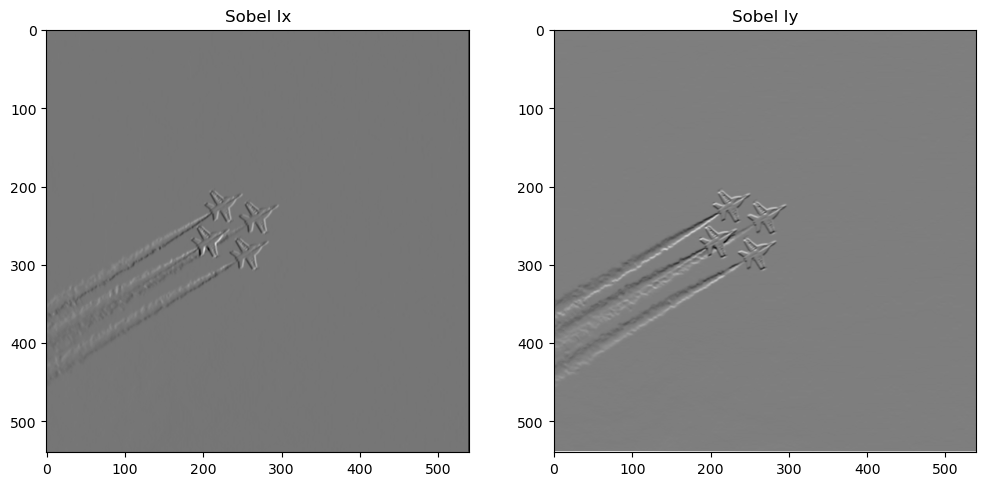
\includegraphics[width=\linewidth]{images/gradients_sample.png}
    \caption{Example of what a sobel kernel applied via convolution to an image in both x then y directions.}
    \label{fig:sobel_gradient}
\end{figure}

\begin{figure}[h]
    \centering
    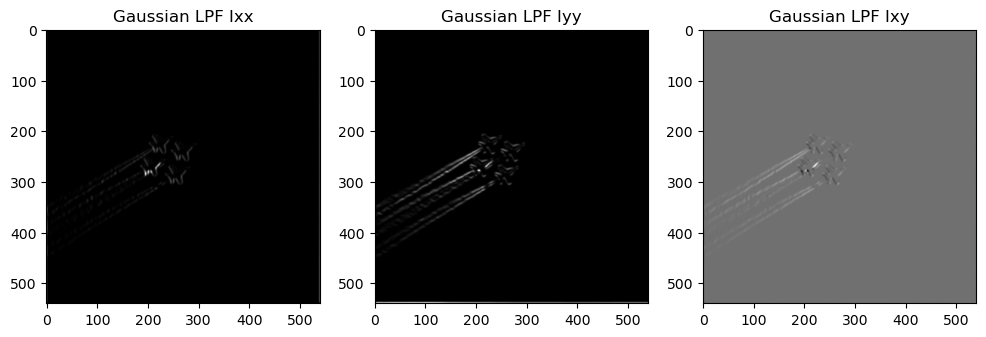
\includegraphics[width=\linewidth]{images/gaussian_low_pass_filters.png}
    \caption{Example of Gaussian low-pass filters applied in the x, y, and xy orientations. The filters smooth the image in the respective directions, reducing high-frequency noise.}
    \label{fig:gaussian_lpf}
\end{figure}

\begin{figure}[h]
    \centering
    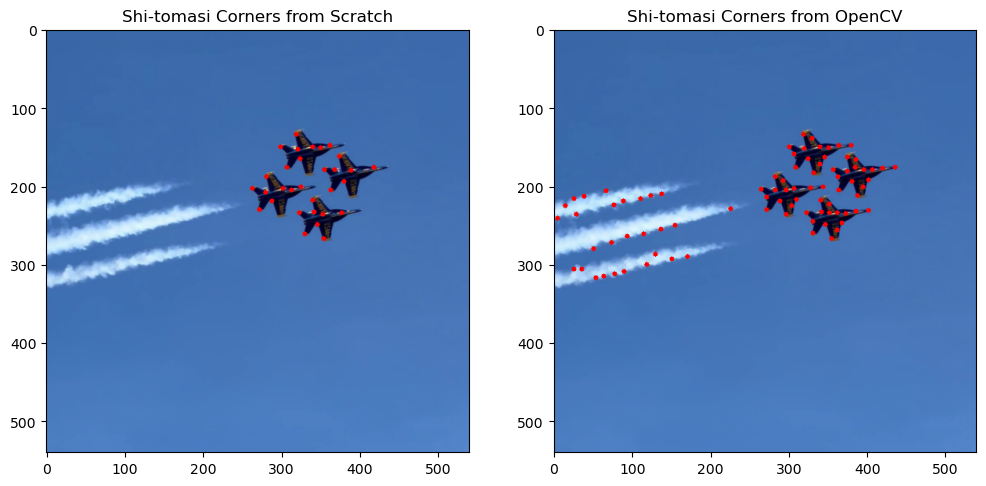
\includegraphics[width=\linewidth]{images/shi_tomasi_corners.png}
    \caption{Detected corners using the Shi-Tomasi method. Left image is pure Numpy implementation, right image is OpenCV's goodFeaturesToTrack method. Red circles indicate detected corners overlaid on the input image.}
    \label{fig:shi_tomasi_results}
\end{figure}


\section{Experimental Results}
[This section will contain your experimental results, with tables and graphs showing the impact of varying parameters such as window size, sensitivity, and threshold values. Discuss the results with respect to accuracy, robustness, and computation time.]

\section{Discussion}
[Analyze the results, comparing performance across parameter variations. Highlight any strengths and weaknesses identified during testing and suggest possible improvements.]

\section{Conclusions and Future Work}
This project demonstrates the practical implementation of the KLT feature tracker, highlighting its effectiveness and limitations. Future work could explore integrating advanced outlier rejection methods or applying the algorithm to large-scale datasets.

\section*{Acknowledgment}
The author would like to thank [Any acknowledgments you wish to include].

\begin{thebibliography}{1}

    \bibitem{ShiTomasi}
    J. Shi and C. Tomasi, "Good features to track," in *Proc. IEEE Conf. Computer Vision and Pattern Recognition*, 1994, pp. 593-600.
    
    \bibitem{LucasKanade}
    B. D. Lucas and T. Kanade, "An iterative image registration technique with an application to stereo vision," in *Proc. Intl. Joint Conf. on Artificial Intelligence*, 1981, pp. 674-679.
    
    \bibitem{OpenCV}
    G. Bradski and A. Kaehler, *Learning OpenCV: Computer Vision with the OpenCV Library*. O'Reilly Media, 2008.
    
    \bibitem{Tan:Digital_Signal_Processing} 
    L. Tan, \textit{Digital Signal Processing}, INAOEP, 2013. [Online]. Available: \url{https://www-elec.inaoep.mx/~jmram/Digital_Signal_Processing__LI_TAN.pdf}.
    
    \bibitem{Wikipedia:KLT} 
    "Kanade-Lucas-Tomasi feature tracker," \textit{Wikipedia}, 2023. [Online]. Available: \url{https://en.wikipedia.org/wiki/Kanade%E2%80%93Lucas%E2%80%93Tomasi_feature_tracker}.
    
    \bibitem{Oppenheim:Schafer} 
    A. V. Oppenheim and R. W. Schafer, \textit{Discrete-Time Signal Processing}, 3rd ed., Pearson, 2010.
    
    \bibitem{KLT:Original}
    C. Kanade, T. Lucas, and B. Tomas, "An improved optical flow algorithm," in \textit{Proceedings of the IEEE Conference on Computer Vision and Pattern Recognition}, 1987, pp. 12-21. [Online]. Available: \url{https://ieeexplore.ieee.org/stamp/stamp.jsp?tp=&arnumber=6716443}.
    
\end{thebibliography}

\end{document}
